\documentclass{apl-guide}
\usepackage{subfiles}
\usepackage{tabularx}
\usepackage{lipsum}
\usepackage{siunitx}
\usepackage[utf8]{inputenc}
\graphicspath{{graphics/}}

\title{Superconductivity}
\experiment{SC}
\course{}
\creation{July 21st}
\author{Rhamel Roomes-Delpeache}
\revisions{}
\owner{University of Toronto}
\labpicture{experiment_graphic.jpg}

\newcommand{\K}{\SI{77}{\kelvin}}
\begin{document}
\maketitle
\tableofcontents
\section{Introduction}
In this experiement you will be looking at the supercoducting properties of
bismuth-strontium-calcium copper-oxide (specifically \ch{Bi_2Sr_2Ca_2Cu_3O_{10+x}} where
$0<x<1$ or BSCCO for short). Superconductivity is a
phenomenom experienced by certain materials, where at certain temperatures,
there is theoretically no electrical resistance. Your job in this lab is to
investigate the validity of the previous statement. During this experiment you
will cover many topic related to experimental physics. You will learn how vacuum
pumps work, take the oppurtunity to connect electronics and perform simple
circuit measurements, calibrate transdiode for temperature measurement, and work
with liquid nitrogen in a cold metal dewar. 

\section{Background}
Superconductivity is the phenomenon that electrical resistance of certain
materials vanishes at low temperatures. It was first discovered in 1911 by Hieke
Kamerlingh Onnes in 1911 which involved the engineering feat of liquifying 
helium (4.2 kelvin). 
The field was revolutionized in 1986 when \emph{high temperature superconductors}
were discovered. These are material who have very low (or vanishing) electrical
resistance at high temperatures, ie $T >> \SI{4.2}{K}$. In this
experiment you will be studying the electrical resistivity of
bismuth-strontium-calcium-copper-oxide (BSCCO) a ceramic material who has
superconductive phase transition above \K \ at ambient pressure.

Here you will be using the 4-wire method to measure the electrical resistivity in
the BSCCO sample. First we will see why this method is necessary, then how it
works, and finally how to implement it. 

\vspace{10pt}
\begin{minipage}{0.8\textwidth}
\textbf{Question:} Suppose we had a sample of pure copper, with a rectangular
cross section \SI{2}{\mm} x \SI{3}{\mm} and length \SI{20}{\mm}. What is the
room temperature reistance of copper, measured from end to end?
\end{minipage}

\vspace{10pt}
\begin{minipage}{0.8\textwidth}
\textbf{Question:} Suppose the electrical connections to this sample-in-dewer
  were established using two phosphor bronze wires of \SI{10}{\mm} diameter,
  that were each half a meter long. What is the resistance of the wires?
\end{minipage}
\vspace{10pt}

As you can see the resistance is dominated by the wires when the resistivity
of the sample is small (as in the case of this experiment). One might try to
measure the resistance of the connecting wires and simply subtract it away from
the measured resistance but this is not as simple as one would expect because the
resitance of the wires are temperature dependent. Changing the material of the
wire or the diameter will ultimitely effect its thermal resistance, leaking
temperature to the outside enviorment. 

To solve the problem we use the \emph{4-wire resistivivty method}. This method
consists of having two seperate pairs of wires connected the the sample. One set
injects, and collects current into the sample while the other is used to measure
the potential difference across a certain portion of the sample
(see figure \ref{fig:4_wire}).
\begin{figure}
  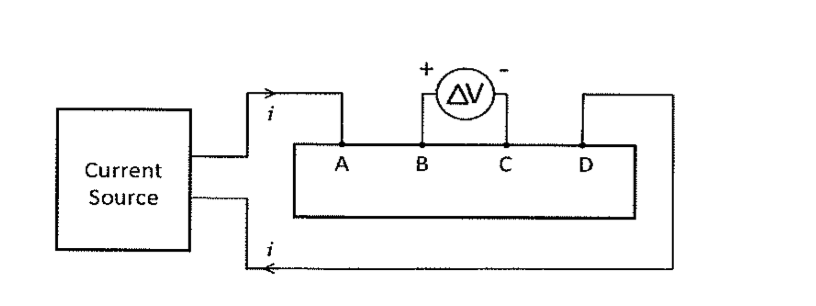
\includegraphics{4_wire_diagram}
  \caption{\label{fig:4_wire} Schematic of a 4 wire measurement}
\end{figure}

In this experiment we will be measuring very small voltages. On the scale of
microvolts, this opens us up to a lot of noise. To combat this we use a lock-in
amplifier to lock on a signal of a specific frequency and phase.
for more information on lock in amplifers see the 
APL youtube page for infromation on lock-in amplifers. 

To measure the resistance we take advantage of \emph{AC ohms law}: 
\begin{equation}
  V_{rms} = Z I_{rms}
\end{equation}

where the subscript \emph{rms} refers to root-mean-square and Z is the
impedance. Z is a complex quantity that comprising of the resistance, $R$, and
reactance, $X$, of a circuit element.

\begin{equation}
  Z = R + jX 
\end{equation}

\textbf{Question:} How will you measure only resistance using the lock in
amplifier?

\section{Activities}
\subsection{Cryostat Exercise}
Read the appendix entry for the cryostat in this manual and complete the tasks
listed.

\subsection{Calibrating Transdiodes}
There are 3 transdiodes in this experiment:
\begin{itemize}
\item Attached to the LN2, this diode give the fastest response to any cooling
  due to the addition of LN2 in the system due to its proximity to the dewer.
\item Attached to the copper baseplate,
\item On the copper plate attached to the sample. 
\end{itemize}
Each transdiode takes a \SI{10}{\uA} current in the forward direction. A higher
current may damage the diode. 

In order to convert the voltage reading of each diode to the correct temperature
reading each transdiode must be calibrated. That is the constants in the curve
\begin{equation}
V(T) = c_1 - c_2T - c_3 ln(T/\SI{1}{\kelvin})
\end{equation}
must be found. As a reminder this is a model of the voltage-temperature
dependence of the transdiode with 3-pt calibration. This curve would have been
introduced in the temperature section of the manual.
To do this you will want to use two known temperatures, and measure the voltage
reading of each diode. You have access to these temperatures. (1) room
temperature and (2) the \K\ of LN2. 

\textbf{Calibrating the transdiode attached to the cryostat.}
While the dewer outer casing has not been
attached use a themometer to measure the surface temperature of the LN2 dewer
and the copper baseplate. This will be your hot point. Note the voltage reading. 
Now with the resevoir closed and at vacuum but the sample not attached, cool the
resevoir down to 77 degrees kelvin. You will know you have reached this
temperature, when the addition of any LN2 does not increase the voltage. This
should be around \SI{990}{\mV} for both transdiodes.

The transdiode on the baseplate will read \SI{990}{\mV} at \K. What does it read
at room temperature?

\textbf{Calibrating the transdiode attached to sample.}
It is your job figure out which wires attached to the transdiode are to
used to inject/eject current and which will be used to measure the voltage. 

\subsection{Controlling the temperature controller}
The goal here is to understrand the servio mechancism of the PI controller and
find the correct time constant at which to set the controller. The transdiode
connected to the PI temperature controller is attached to the copper baseplate
of the LN2 resevoir. Put the system under vacuum and cool it to \K. With the DC
power supply \emph{off}, the gain on the PI controller set to 1, and the time
constant toggle set to off. (Note: all the signals on the PI controller analog
outputs are 10x the real signal amplitude.) Rotate the \emph{set temp} knob such that the
anolog output reads \SI{9.90}{\V}. The error LED should be green. Keeping the DC
power supply off, rotate the knob such that the set temperature anolog output is
\SI{9.85}{\V}, using the oscilliscope keep track of the error and temperature
analog outputs to see how these values change. 

Now when the anolog output of the set temperature diode and the temperature
diode match: increase the gain dial to a value of 5 or more and decrease the set
temperature by another \SI{0.05}{\V}. Repeat this process untill you see an
overshoot in the temperature analog output as the PI controller tries to match
the temperature of the set point. If you do not see an overshoot you should see
a gain. 

Now flip the switch on the gain control to x10. Starting at a modest gain value
of 1 (this is actually a x10 gain) decrease the set point temperature again by
\SI{0.05}{\V}. Continue this process of increasing the gain then decreasing the
temperature until you not only see an overshoot but an oscilation in the
temperature anaolog output around the the set temperature. Mark down the gain
setting where this is achevied. The period of the oscillation is the time
constant for the system. Adjust the time constant settings accordingly and
decrease the gain slightly.

With the output of the DC power supply still off set the voltage to
\SI{60.0}{\V} and the current limit to \SI{1.0}{\A}. Connect the ouptut of the
DC power supply to the back of the PI controller using banna plugs. The PI
controller is now ready to be used. 


\subsection{Testing your method}
To ensure that you understand how to correctly measure the resistance of the
sample you will test out the method with a breadboard and resistor (ideally
\SI{0.1}{\ohm}, why?). Complete a setup as shown in figure \ref{fig:4_wire}.

Using the coil driver module, inject a \SI{100}{\mA} AC current into circuit.
The coil driver has two anolog connectors on its front pannel. The first
\emph{osc. in} controls the amplitude and frequency of the generated current.
Using a function generator, you send the signal through this anolog channel. The
coil driver will then output a AC current from its rear panel the is $1/10$ the
amplitude of the voltage signal but at the same frequency and phase. 
The second \emph{mon. out} gives you a way to view the the generated current.
\emph{mon, out} passes the current over a \SI{1.0}{\ohm} resistor to generate a
voltage of the same frequency and amplitude as the current. This can be viewed
by connecting a BNC cable to one of the oscilliscope channels. 

The lock-in amplfer used in this experiment has a built in function generator.
It is best to use this generator to power the coil driver. 

First, using the controls on the front panel of the lock-in amplifier set the
internal oscillator frequency to \SI{37.0}{\hertz}. Note, lock-in amplifers
display the root-mean-square voltage ($V_{rms}$). Where:
$$V_{rms} = 1/\sqrt{2} V \text{    or     } V_{rms} = 1/(2\sqrt{2}) V_{pp}$$
and $V_{pp}$ is the peak-peak voltage. Set the oscillator amplitude such that
the output current generated by the coil driver will be \SI{100}{\mA}.

Using a BNC connector, connect the \emph{osc. out} analog channel on the lock-in
to the \emph{osc. in} on the coil driver. Use \emph{mon. out} and the
oscilliscope to ensure that the current you are generating is the what you
expect.

\textbf{NOTE:} In order for \emph{mon. out} to output the signal the coild
driver must be driving a circuit. Ie you must connect in the the breadboard and
have it drive a load (the resistor) for a current to actually be generated. The
output of the driver is two banana jacks on the rear panel of the coil driver
module-in to the \emph{osc. in} on the coil driver. Use \emph{mon. out} and the
oscilliscope to ensure that the current you are generating is the what you
expect.

\textbf{NOTE:} In order for \emph{mon. out} to output the signal the coild
driver must be driving a circuit. Ie you must connect in the the breadboard and
have it drive a load (the resistor) for a current to actually be generated. The
output of the driver is two banana jacks on the rear panel of the coil driver
module.

Now use the lock-in amplifer to pick up the voltage across the resistor. Is the
value what you expect?

\subsection{Complete a run}
With the above complete you are now ready to run your system. Make sure that you
read the README.md file provided with the code for the experiement to understand
how to take data. 
\begin{enumerate}
  \item Attach the sample to the nickle-plated copper baseplate. 
  \item Thermal contact between the baseplate and the sample is created by
    clamping tightly screwing the brass bolts onto the baseplate. 
  \item Close the system ensuring that all the electronics are properly working. 
  \item Power the PI controller using the DC power supply.
  \item Use the code provided to run the system to some set temperature, and
    choose the sample rate.
  \item Save the data as needed. 
\end{enumerate}

To cool the system simply turn off the heating resistors and add LN@ if needed. 

\subsection{Things to look for}
\begin{enumerate}
  \item The phase transition is not a sharp spike, but a slope. Find the width
    of the slope. 
  \item What are the effects of changing the sampling rate?
  \item Try running the system such that the sample is at ambient pressure. Try
    again with it at vacuum. Are there a difference in your results?
\end{enumerate}

\section{Appendix}
\subfile{cryostat.tex}
\end{document}

